\subsection{Verification and Validation on Event-B models}

The Event-B method share the same language than the classical  B method. Besides both approaches are based on a pre/post -condition mechanism to describe the evolution of the system. Thus similar verification mechanisms can be defined.


\subsubsection{Verification Processes Applicable to Event-B}
\label{sec:verif-proc-appl}

An Event-B model is a formal specification that describes the functional
behavior of a system from a global point of view. In general, an Event-B model
comprises a set of state variables, parametrized events that can modify these
state variables and invariants that describe logical properties thereof.  The
invariants are in first-order predicate logic and can be discharged using
different proof engines, e.g.,\  automatic modern open source SMT solvers and
manual predicate provers.

In general, one starts with a rather abstract description of the model which is
iteratively refined until the desired level of detail is reached. Event-B
supports this refinement by creating the necessary proof obligations that ensure
correct refinement in each step, both for behavioral refinement of events as
well as for data refinement of state variables.

Thanks to the integration into the Eclipse platform, there are many plug-ins
available as extensions. There is a plug-in to use graphical modeling in UML
state machines to describe Event-B models. There is a tight connection to the
ProR requirements engineering plug-in. To facilitate modeling, there are
plug-ins to decompose a model into several sub-models and to facilitate proving
by supporting external formal theories.

Together with the Rodin tool, the Event-B approach was developed in the European
research projects RODIN (2004--2007) and DEPLOY (2008--2012). Since 2011 it is
further developed in the European project ADVANCE\@.

\paragraph{Verification of Type Safety}
\label{sec:verif-type-safety}

Static type checking is a technique that allows the verification of correct
typing for variables at compile / modeling time. It is performed after lexical
and syntactic correctness of the Event-B model have been verified. Static type
checking prevents all type errors at run-time, which eliminates many possible
sources of program errors.

The type system of Event-B is much more expressive than the one of most other
languages, as Event-B also allows the usage of dependent types for variables. In
this case, the type of a variable is dependent of its value, e.g.,\ one can
define the type of all even integers. Event-B can define such types and verify
that events respect the correct dependent typing of variables

In Event-B, every new variable gets a type assigned via a typing invariant. Such
an invariant is either an explicit type assignment or an implicit one, e.g.,\ by
specifying a dependence to another variable which is typed. The integrated type
interference can then deduce the static type of the new variable.

Every event that changes the value of a variable via substitution must also
respect the variable typing. For each event that modifies a variable,  proof
obligations are created that ensure this in a rigorous formal way.

In almost all cases, the proof obligations for type verification are discharged
automatically by the Rodin provers.

\paragraph{Verification of Well-Definedness}
\label{sec:verif-well-defin}

After type checking, one or more well-definedness (WD) proof obligations are
created. This ensures that the expression has a unique meaning and prevents the
usage of expressions that make no sense or are ambiguous.

One prominent example for WD proof obligations in Event-B is the cardinality of
sets. The set of natural numbers $\mathbb{N}$ has countable infinitely many
elements, exactly as many as the set of all even natural numbers
$\mathbb{N}_2:=\{2\cdot n \mid n \in \mathbb{N}\}$. This means that both sets
have the same cardinality, although $\mathbb{N}_2$ is a strict subset of
$\mathbb{N}$.

Therefore, while sets of countable infinite cardinality can be used without any
problem in Event-B models, the usage of cardinality of a set requires the set to
be of finite size which gets verified by an appropriate WD proof obligation.

In almost all cases, the proof obligations for well-definedness are discharged
automatically by the Rodin provers.


\paragraph{Model Simulation}
\label{sec:model-simulation}

A correctly typed Event-B model can be simulated or animated using different
plug-ins like AnimB or ProB. At each step, one of the activated events can be
executed and if applicable parameters for that event can be defined. This allows
for stepping through the formal model, observing the state variables and the
invariants. Using model animation, it is possible to validate the correct
functioning of the model.

\begin{figure}[ht]
  \centering
  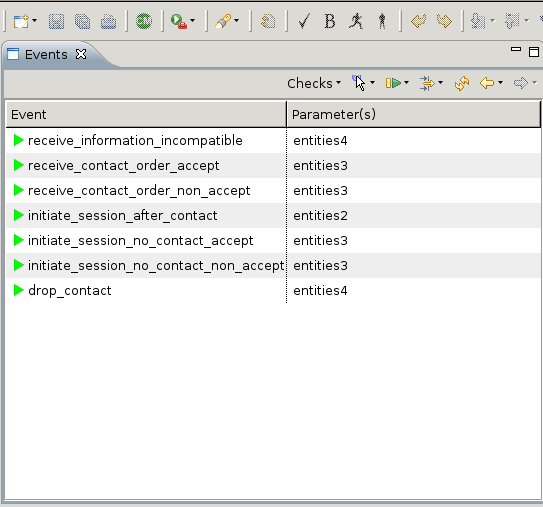
\includegraphics[width=.5\textwidth]{figures/ProBAnimation}
  \caption{ProB Model Animation}
  \label{fig:proBAnimation}
\end{figure}

Figure~\ref{fig:proBAnimation} shows a ProB simulation session. The activated
events are marked green, clicking on them allows for selection of parameters and
to execute the events with the chosen parameters.


\paragraph{Model-Checking of Predicates}
\label{sec:model-check-pred}

Model-checking is a static analysis of the semantics of a model. In general, a
model-checker will create a representation of the whole possible state space of
a model and verify logic properties on this state space. There are many
different possibilities for properties that are verified by model-checkers, some
are listed here:

\begin{itemize}
\item {\bf Equivalence Checking} The equivalence between two models is verified
  given a certain equivalence relation. Often, a specification is compared to
  its (distributed) implementation using bisimulation modulo some reduction
  techniques, e.g.,\ only the externally observable behavior is compared and the
  internal details of the different systems are ignored.
\item {\bf Deadlock Freeness} A deadlock represents a state where the system
  that the system cannot leave as no event is enabled. For a reactive system
  this is always an unwanted state that must be avoided.
\item {\bf Temporal Properties} The evolution of the system over time is
  analyzed, i.e., the admissible event sequences that can lead to different
  states. Roughly, temporal properties comprise \emph{safety properties} which
  describe a set of states that should never be reached and \emph{liveness
    properties} which describe states that should always be reachable. There are
  different temporal logic languages, like LTL and CTL, which allow to describe
  temporal properties of systems.
\end{itemize}

In general, model-checkers suffer from the state space explosion problem. This
means that creating the whole state space becomes often infeasible due to memory
limitations. In general it is also not possible to model-check systems with
infinite state space, like many Event-B models.

In practice, tools like ProB which allow for model-checking of Event-B models,
limit the size of the possible values for variables to a finite subset. While
this means that a complete proof is not possible, it allows for fully automatic
error detection in the model. For any violated property or a deadlock, ProB
provides a counterexample that can be analyzed and therefore allows for
correction of the associated modeling problem.

\begin{figure}[ht]
  \centering
  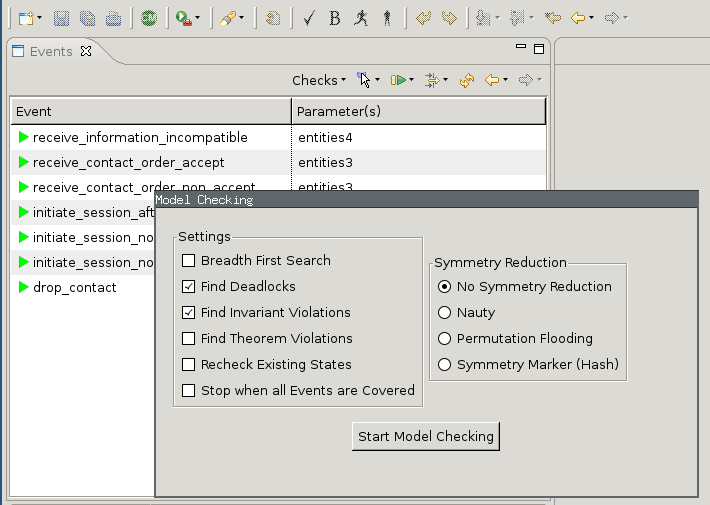
\includegraphics[width=.5\textwidth]{figures/ProBModelChecking}
  \caption{Model-Checking for Deadlocks}
  \label{fig:Prob-model-check}
\end{figure}

Figure~\ref{fig:Prob-model-check} shows the model checking dialog of the Rodin
plug-in for ProB. The currently selected options would check for deadlocks,
i.e.,\ a sequence of events that leads to a situation where no event can be
selected anymore.


\paragraph{Formal Proof of Predicates}
\label{sec:form-proof-pred}

Formal proof techniques provide a much more powerful way to verify predicates
than model-checking. Instead of the creation of the full state-space, they use a
proof calculus to iteratively simplify predicates and to reduce them onto known
lemmas or axioms, thus discharging them.

In contrast to model-checking, formal proof is applicable to models of infinite
size and can cope with undecidable problems. Although this means that there
sometimes will be a manual step in a proof, there are many automated tools that
support formal proofs and can often discharge proof obligations without any
manual intervention.

The Rodin platform natively supports manual construction of formal proofs by
allowing easy access and manipulation of the proof tree and predicate
hypotheses. It also provides access to different automated provers, i.e.,\ the
free of charge AtelierB provers, an open source SMT plug-in that supports
several solvers\footnote{supported open source SMT solvers include: verIT,
  Alt-Ergo, CVC3, Z3} as well as an open source plug-in that connects Rodin to
the Isabelle/HOL proof assistant.

\begin{figure}[ht]
  \centering
  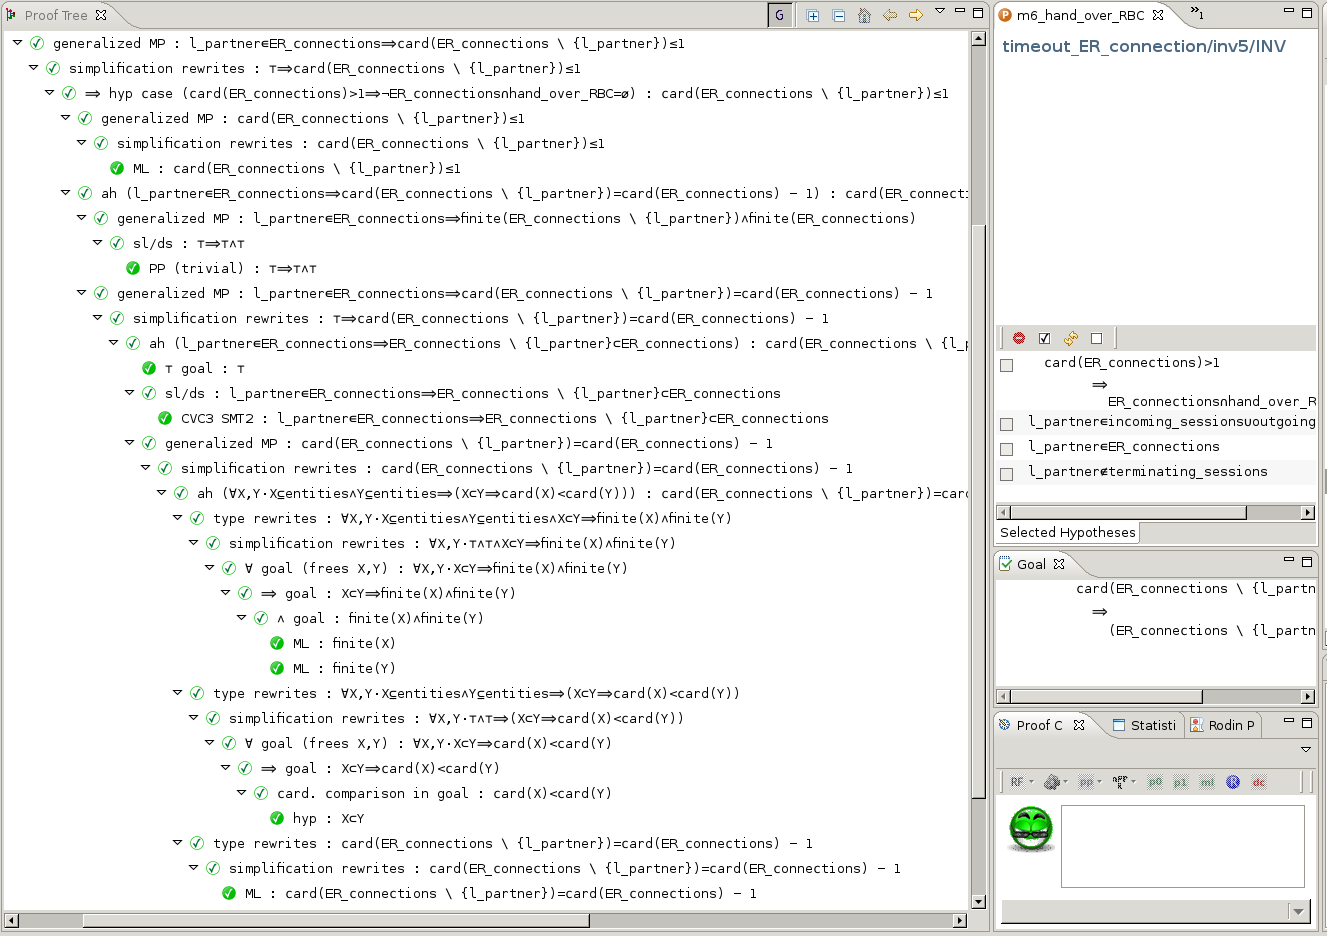
\includegraphics[width=1\textwidth]{figures/ProofTree}
  \caption{Rodin Proof Tree}
  \label{fig:proof-tree}
\end{figure}

Figure~\ref{fig:proof-tree} shows a part of a Rodin proof tree for an
invariant. Its green color signals that the proof is finished, at each node in
the tree, the applied proof rule is shown. This allows for easy inspection of
the proofs and allows both for humans and for machines to verify the correctness
of the proof steps.


\paragraph{Verification of Refinement Correctness}
\label{sec:verif-refin-corr}

Rodin provides extensive support for a top-down development approach and allows
for an iterative refinement of models. The model is developed using different
levels of detail, starting from a rather abstract view, refining the details
where necessary or desired. This refinement process can either be applied to
the events or the variables.

\subparagraph{Data Refinement}
\label{sec:data-refinement}

In general, a data refinement replaces a variable with another one, or multiple
other ones. For example a Boolean variable in the abstract model is replaces by
an enumeration with different possible values. To ensure a correct refinement,
one has to manually supply a ``gluing'' invariant that describes the connection
of the refined and the abstract variable. For example one subset of the possible
values for the enumeration in the refined model would correspond to a value of
``True'' in the abstract model, the remaining values of the enumeration to a
value ``False''. The abstract variable is then deleted from the refined model,
and the necessary proof obligations are created automatically by Rodin.


\subparagraph{Code Refinement}
\label{sec:code-refinement}

For event (or code) refinement, Rodin automatically creates the necessary proof
obligations that ensure that the abstract system is correctly refined by the
more detailed model. This includes the verification that each refining event
only modifies variables that are also modified by the abstract event and that
the modification is equivalent. It also includes verification of guard
strengthening, i.e.,\ the guards of a refining event must be at least as
constraining as of the refined abstract event. A common code refinement is to
split an event in several more specialized ones, where the additional guards
ensure mutual exclusion of the activation conditions.

\begin{figure}[ht]
  \centering
  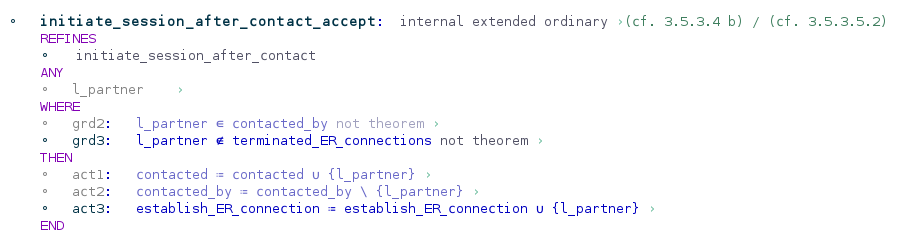
\includegraphics[width=.9\textwidth]{figures/EventRefine}
  \caption{Event Refinement}
  \label{fig:event-refine}
\end{figure}

Figure~\ref{fig:event-refine} shows a refining event with guard strengthening
and an additional variable that is modified. The pale blue colored guards and
actions are derived from the refined event, the darker colored guard and action
are the additional ones for the refining event.


\paragraph{Verification of Design Step Requirements}
\label{sec:verif-design-step}

This section reports on the verification activities of the correct
implementation of the design step requirements. The goal of the activity is to
establish a correct formal representation of the design step requirements.

The activity is described in the Verification and Validation
Plan~\cite{vnvplan}.  In short, it consists of formalizing and proving the
identified requirements of a preceding phase, to ensure their correct
implementation of the requirements. To achieve this, we use the direct
connection between the Event-B model and the ProR based on an EMF model of the
Event-B model.


\paragraph{Verification of Safety Requirements}
\label{sec:verif-safety-requ}

A safety analysis identifies additional requirements which guarantee the safety
of a system. It must be verified that the system model correctly implements
these non-functional requirements. Not every safety requirement is applicable on
the system development level. Many are on the implementation level, e.g.,\ they
demand that certain safety-critical functions are done in a redundant way to
reduce the risk of malfunctioning or loss of that function.

In the safety analysis~\cite{safetyBrice}, a list of safety requirements was
identified using an FMEA analysis of the communication system. A ReqIf file
captures all these safety requirements within ProR, the concerned functional
requirements are traced in the ReqIf file for Subset-026 chapter 3.5.

Each of the safety requirements is examined for applicability in the system
level model, the identified ones are formalized. Most often, the safety
requirements are represented as one or more additional invariants in the system
model. These invariants are linked to the ReqIf file that describes the safety
requirements, ensuring traceability in the model.

\begin{figure}[ht]
  \centering
  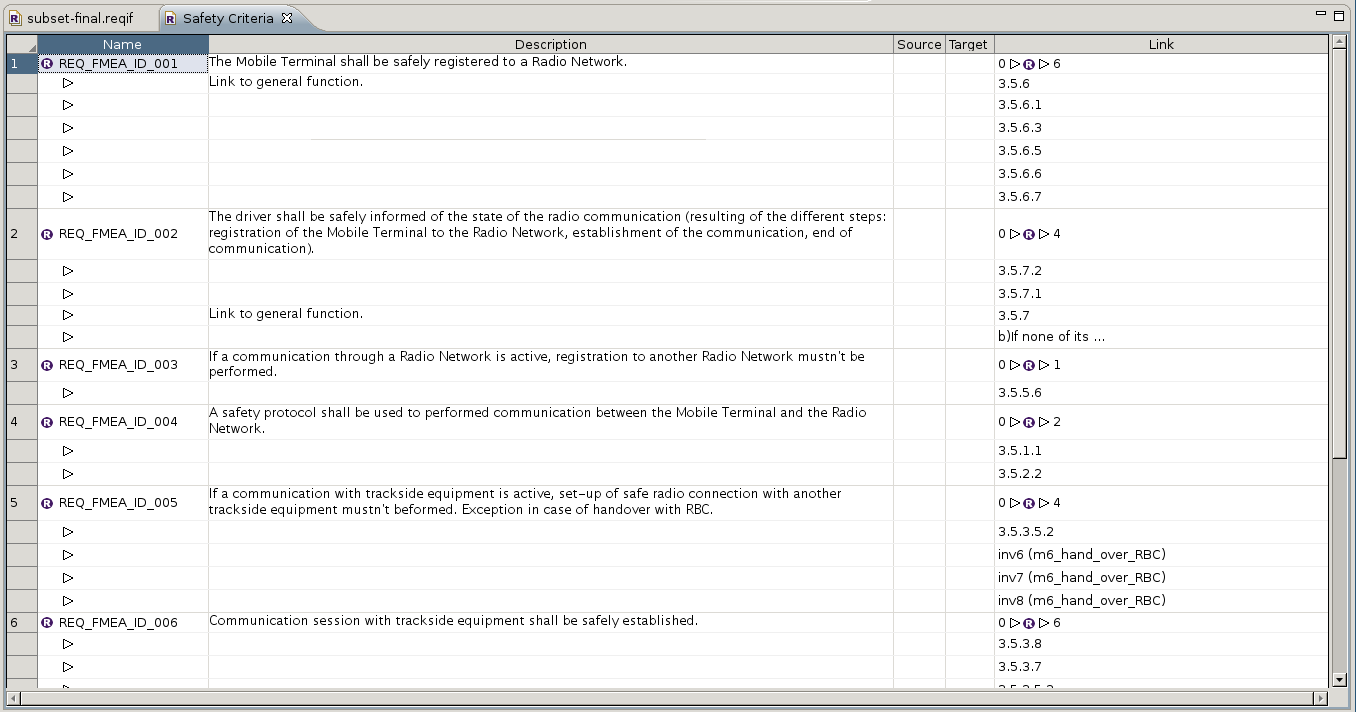
\includegraphics[width=1\textwidth]{figures/ProRSafetyReq}
  \caption{Safety Requirements}
  \label{fig:pror-safety-req}
\end{figure}

Figure~\ref{fig:pror-safety-req} shows a ReqIf document in Rodin (via the ProR
plug-in) which holds the safety requirements defined by the safety analysis. For
each requirement, there are references to the concerned elements of Subset-026 and
to Event-B elements where applicable, e.g.,\ {\sf REQ\_FMEA\_ID\_005} which is
linked to the invariants, {\sf inv6}, {\sf inv7} and {\sf inv8}.


\paragraph{Verification of Requirements Coverage}
\label{sec:verif-requ-cover}

This section reports on the verification activities of the coverage of the
design step requirements. The goal of the activity is to establish the coverage
degree of the formal representation of the design step requirements.

The activity is described in the Verification and Validation
Plan~\cite{vnvplan}.  In short, in consists of analyzing the coverage of the
identified requirements of a preceding phase, to ensure their completeness of
implementation of the requirements wrt.\ the refinement level of the model. To
achieve this, we use the direct connection of the Event-B model with the ProR
based on an EMF model of the Event-B model.


\subsubsection{Object of Verification}
\label{sec:object-verification}

The object of verification is the Event-B model for the communication
establishing at {\url{https://github.com/openETCS/model-evaluation/tree/master/model/Event_B_Systerel/Subset_026_comm_session}}. It
is from the strictly formal modeling phase and represents the communication
session management of the OBU\@.

\paragraph{Available Specification}
\label{sec:avail-spec}

The model implements the requirements for the communication session management
as described in Subset-026 chapter 3.5.

This section describes the establishing, maintaining and termination of a
communication session of the OBU with on-track systems.

%\subsubsection{Detailed verification plan}
%\label{sec:deta-verif-plan}

\paragraph{Goals}

One goal is the development of a strictly formal, fully proven model of the
communication session management and to provide evidence of covering the
necessary requirements of Subset-026 as well as proving correctness of the model
wrt.\ the requirements and attaining a good coverage of the model wrt.\ the
requirements.

The second goal is to correctly implement the applicable safety requirements
identified by the safety analysis. Both functional and safety requirements
should be traced in the model and a requirement document in a standardized
format.

The formal model will represent the described functionality on the system level,
the correct functioning can be validated by step-wise simulation and
model-checking of deadlock-freeness.


\paragraph{Method/Approach}
\label{sec:methodapproach}

At first, the basic functionality described in the chapter 3.5 that are
identified. These serve as basis for a first abstract model, which is refined
iteratively, adding the desired level of detail. The elements of Subset-026 are
traced using links from Event-B to the ProR file in ReqIf format. Requirements
are formalized as invariants and proven where applicable.

\paragraph{Means}
\label{sec:means}

The means used are:
\begin{itemize}
\item open source Rodin tool (\url{http://www.event-b.org/}), including plug-ins
  (for details
  see~\url{https://github.com/openETCS/model-evaluation/blob/master/model/Event_B_Systerel/Subset_026_comm_session/latex/subset_3_5.pdf})
\item ProR requirements modeling tool~\url{http://www.pror.org}
\item open source ProB model checker and B model
  simulator~\url{http://www.stups.uni-duesseldorf.de/ProB/index.php5/Main_Page}
\item open source CVC3 (\url{http://www.cs.nyu.edu/acsys/cvc3/}), verIT
  (\url{www.verit-solver.org}) and Alt-Ergo (\url{http://alt-ergo.lri.fr}) SMT
  solvers
\end{itemize}

% \subparagraph{Other}

%  \bgcmmnt{optional, might be renamed}

\paragraph{Results}
\label{sec:results}

\begin{itemize}
\item The result is a fully formal model of the communication session management
  as described in chapter 3.5 of Subset-026.
\item Each implemented element of this section is linked to the ProR
  requirements file, both specification elements that describe how something has
  to be done, as well as requirements that describe what must be achieved.
\item The model can be simulated / animated, either with the AnimB or the ProB
  plug-in, validating the functional capabilities.
\item The safety requirements are formalized as invariants in predicate logic,
  their proofs are for the most part fully automatic.
\item It was found that while the Subset-026 communication management explicitly
  allows multiple communication partners (see RBC handover), there is no
  explicit limit of established communication connections given in chapter 3.5.
\item A complete covering of the elements of Subset-026 was not realized, e.g.,\
  there is a representation of the contents of a message, but its explicit
  format is not implemented. This is considered an implementation detail without
  influence for a system level analysis. In general, Event-B models will not be
  refined up to the implementation level.
\end{itemize}

\paragraph{Summary}

The created fully formal functional model allows for formalization and proof of
Subset-026 requirements. The integration of Rodin into Eclipse provides easy access
to extensions like the ProR requirements tool which allows for validation of
coverage of requirements.

The integration of various provers, in particular the SMT plug-in automates a
large part of the formal verification. For the model of the communication
management, from 382 non-trivial\footnote{many WD proof obligations are so
  trivial that they will not be shown in Rodin} proof obligations, only 12,
i.e.,\ $3.2\%$ require any manual intervention.

\paragraph{Evidence produced}
\label{sec:evidence-produced}

The formal Event-B model, including a ReqIf document for chapter 3.5 of Subset-026
and a pdf documentation of the model can be found at
\url{https://github.com/openETCS/model-evaluation/tree/master/model/Event_B_Systerel/Subset_026_comm_session}

\subsubsection{Conclusions/Lessons learned}

Having an abstract formal model of the implemented functionality which can be
simulated, allows for interesting insights into the overall functioning of a
system. Formalized requirements are very helpful in both the identification of
ambiguous requirements and in their clarification.

The elements of Subset-026 are of very different nature. Some describe rather
low-level specification details, other describe ``real'' requirements. Without
an analysis as done with this Event-B model, it can be difficult to decide which
elements must be considered on a system level analysis and which on the lower
implementation level.


\subsubsection{Future Activities}
\label{sec:future-activities}

For other sections of Subset-026, that describe a functionality in a way that can be
captured in an iteratively refined model and which has interesting requirements
on a rather high level, creating an Event-B model can provide insight into the
functioning, identify ambiguous or erroneous elements in the specification and
can provide the basis for logical pre- and post conditions of the later
implementation.

